\paragraph{Brechungsindex} $n_D(\SI{20}
{\degreeCelsius}) = 1.5343$ (Lit.: 1.535) \cite{SA1}.

\paragraph{NMR}
$^1$H-NMR (\SI{250}{\mega\hertz}, CDCl$_3$): $\delta$ = 7.64 (d, $^3J$ = \SI{8.5}{\hertz}, 1H, H-2), 7.10 -- 7.03 (m, 2H, H-3, H-5), 2.56 (s, 3H, H-10), 2.52 (s, 3H, H-8), 2.35 (s, 3H, H-7).

\begin{figure}[H]
    \centering
    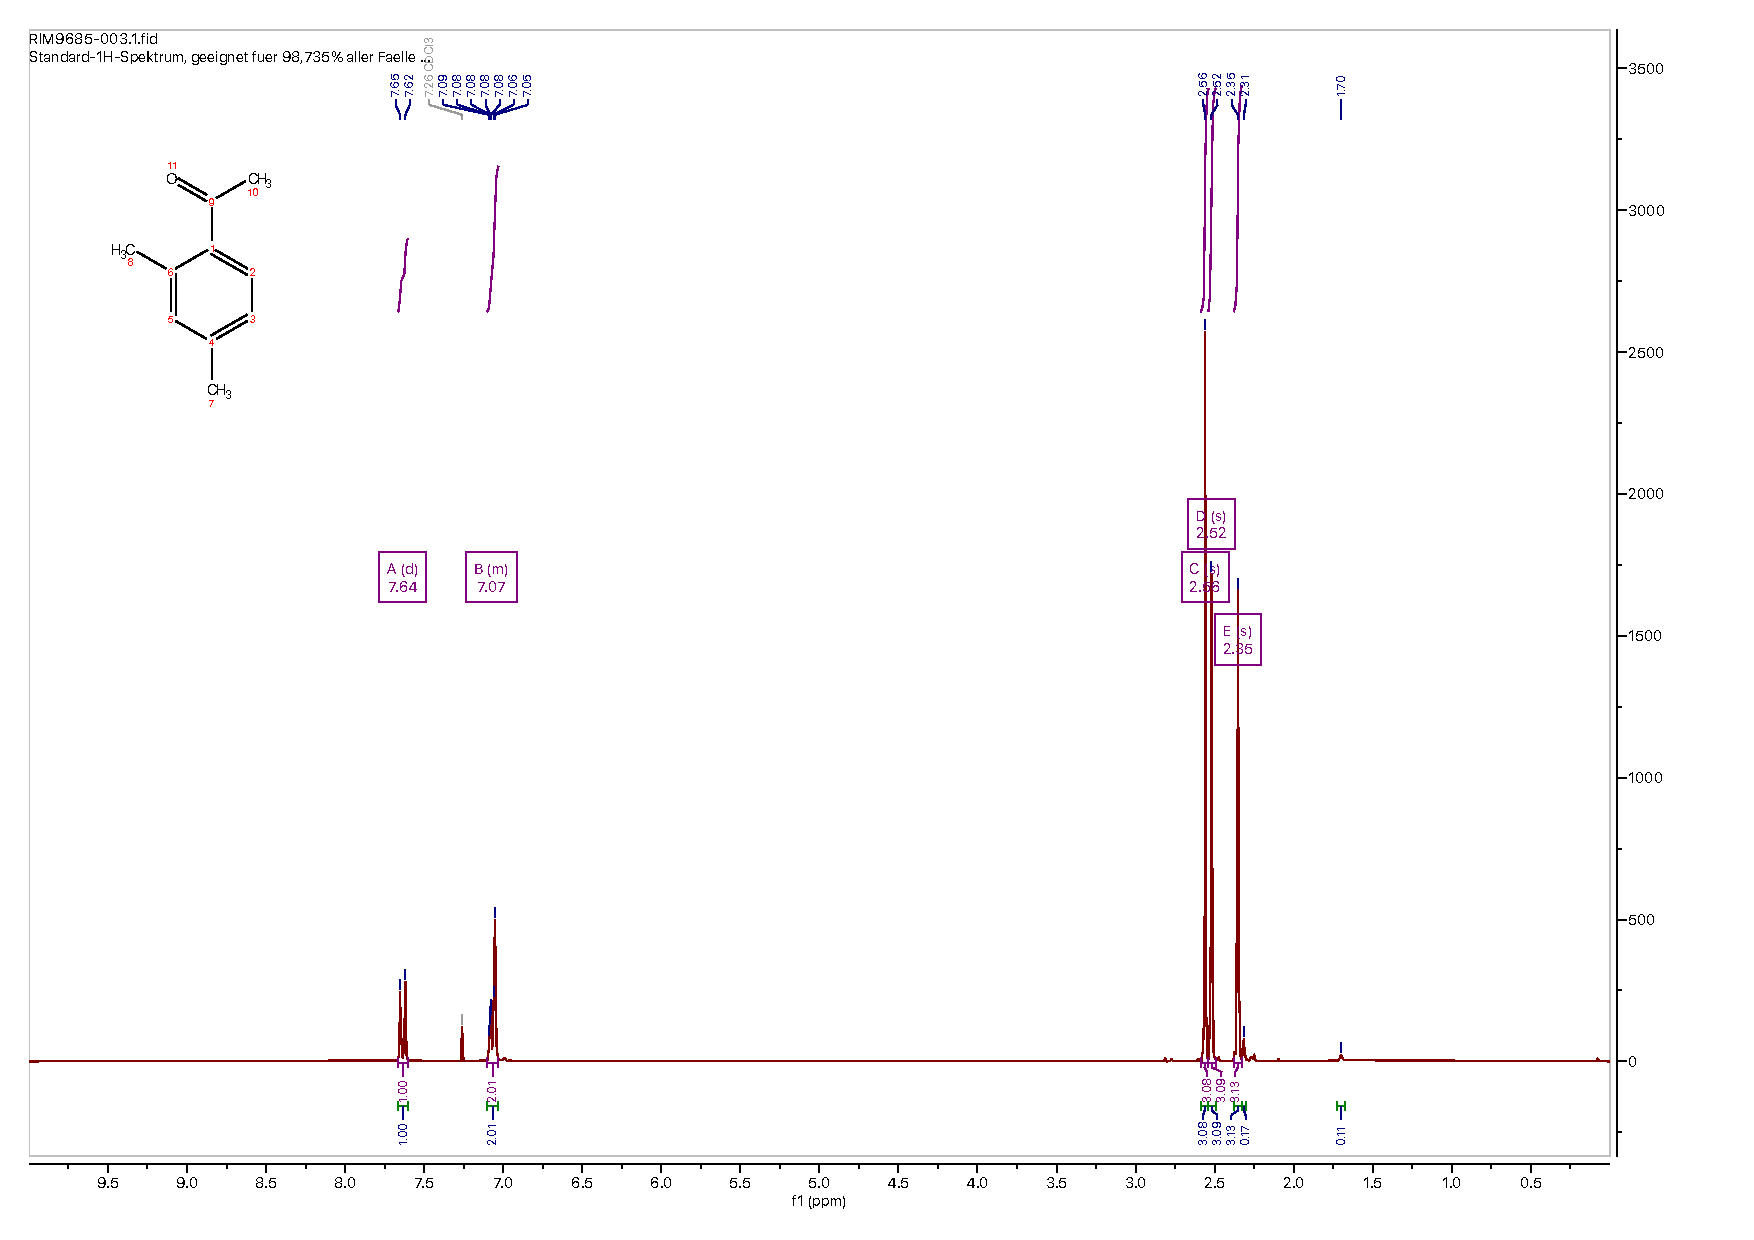
\includegraphics[width=1.0\textwidth]{data/P1_NMR.pdf} \\ [0.5cm]
    \caption{$^1H$-NMR Spektrum des erhaltenen Produkts 2,4-Dimethylacetophenon}
    \label{fig:P1_NMR}
\end{figure}

\paragraph{IR}
Das IR-Spektrum (Abbildung \ref{fig:P1_IR}) bestätigt die Struktur des erwünschten Produkts und passt zur Literatur \cite{SA2}.
Charakteristisch ist die intensive Carbonyl-Valenzschwingung bei $1675\,\text{cm}^{-1}$. Weitere signifikante Signale finden sich bei $2973$ und $2924\,\text{cm}^{-1}$ (aliphatische $C-H$-Valenz-schwingungen) sowie bei $1610$ und $1565\,\text{cm}^{-1}$ (aromatische $C=C$-Gerüstschwingungen). Die starke Bande bei $813\,\text{cm}^{-1}$ ($C-H$ out-of-plane) ist zudem typisch für einen 1,2,4-trisubstituierten Aromaten.


\begin{figure}[H]
    \centering
    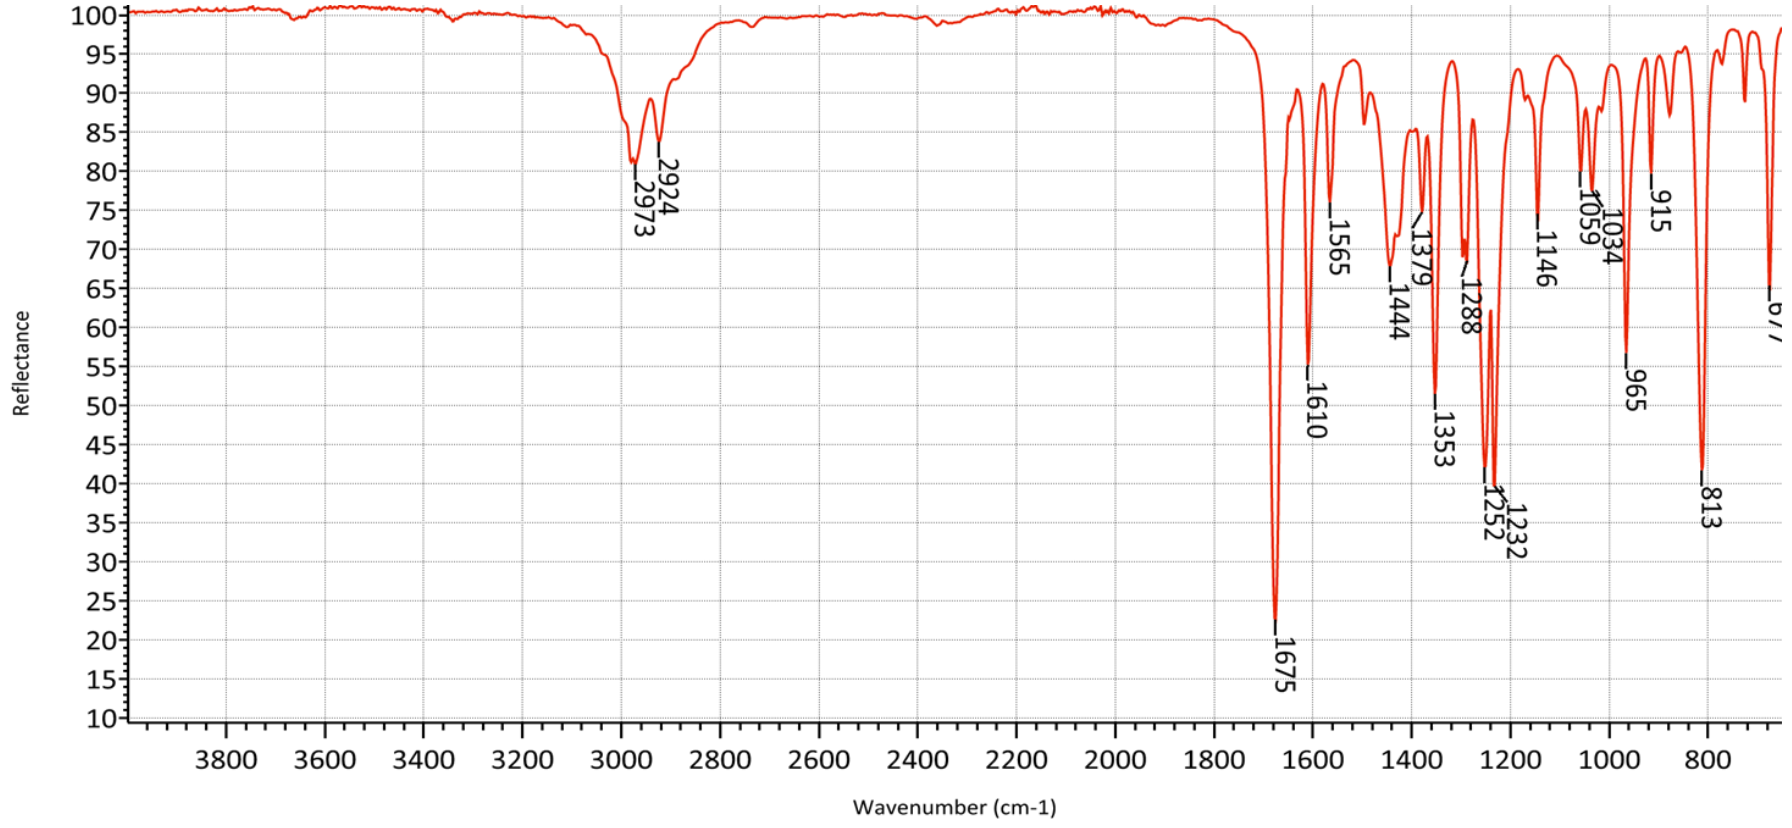
\includegraphics[width=1.0\textwidth]{data/P1_IR.png} \\ [0.5cm]
    \caption{
    IR (2,4-Dimethylacetophenon): $\tilde{\nu}$ ($\text{cm}^{-1}$) = 2973, 2924 (aliph. $C-H$), 1675 ($C=O$), 1610, 1565 (aromat. $C=C$), 813 (aromat. $C-H$).}
    \label{fig:P1_IR}
\end{figure}
